\documentclass{article}
\usepackage{pgfplots}
\pgfplotsset{compat=1.18}

\begin{document}

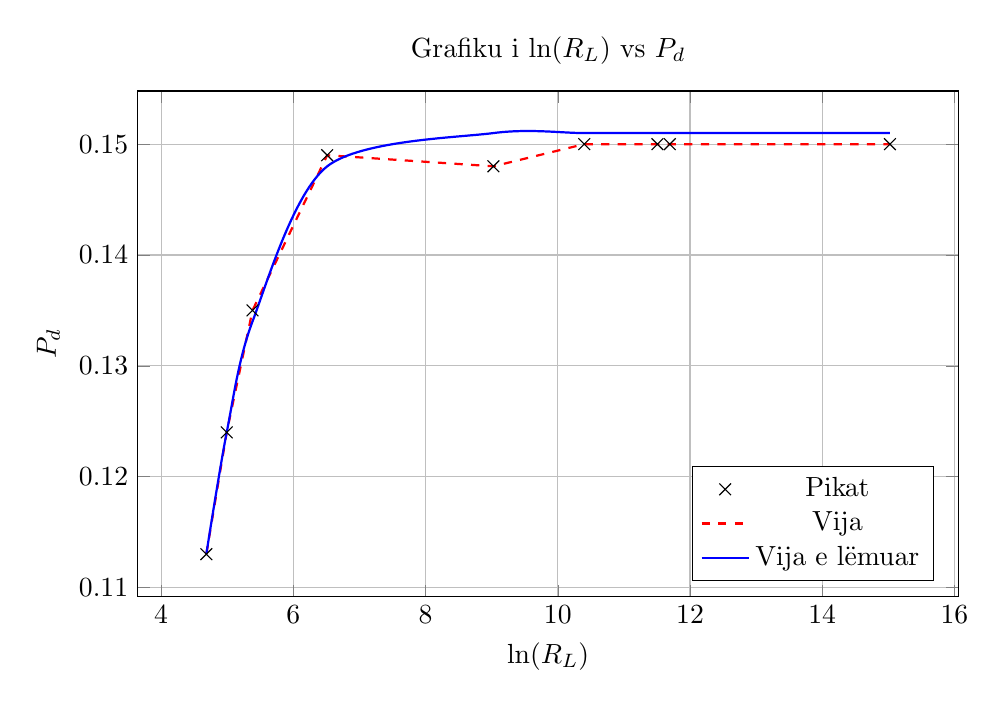
\begin{tikzpicture}
    \begin{axis}[
        xlabel={$\ln(R_L)$},
        ylabel={$P_d$},
        title={Grafiku i $\ln(R_L)$ vs $P_d$},
        grid=major,
        legend pos=south east,
        width=12cm,
        height=8cm
    ]
    
    %Data points
    \addplot[
        only marks, 
        black, 
        mark=x,
        mark size=3pt,
        mark options={solid}
    ] coordinates {
        (4.683, 0.113)
        (4.992, 0.124)
        (5.382, 0.135)
        (6.512, 0.149)
        (9.026, 0.148)
        (10.401, 0.150)
        (11.507, 0.150)
        (11.695, 0.150)
        (15.024, 0.150)
    };
    \addlegendentry{Pikat}
    
    %Dashed line
    \addplot[red, dashed, thick] coordinates {
        (4.683, 0.113)
        (4.992, 0.124)
        (5.382, 0.135)
        (6.512, 0.149)
        (9.026, 0.148)
        (10.401, 0.150)
        (11.507, 0.150)
        (11.695, 0.150)
        (15.024, 0.150)
    };
    \addlegendentry{Vija}

    %Smooth line 
    \addplot[blue, smooth,thick] coordinates {
        (4.683, 0.113)
        (4.992, 0.124)
        (5.382, 0.134)
        (6.512, 0.148)
        (9.026, 0.151)
        (10.401, 0.151)
        (11.507, 0.151)
        (11.695, 0.151)
        (15.024, 0.151)
    };
    \addlegendentry{Vija e lëmuar}

    \end{axis}
\end{tikzpicture}
\end{document}